\section{实验分析}

% 5 页

为了验证和展示本文所提出的模型的有效性和准确性,本文将在这一节设计几个实验,并且根据任务的目标获取与之对应的数据集,从不同规模和结构的数据集上对模型进行评估,随后对模型进行消融实验和参数分析,以确定模型的各步骤的有效性,最后通过真实网络环境下的路由劫持对模型进行案例分析。

\subsection{数据集设置}

由于模型要求输入未经修改的路由路径,本章节的实验将根据具体需求使用来自互联网(RIPE RIS) 和 DN42 两种分布式网路的数据,这两类数据集在数据规模、复杂度和结构特点上有所不同,在先前章节的表 \ref{dataset-compare} 展示了数据集的基本统计信息,对于本章的模型而言,其中最重要的信息为数据集内路由路径的数量和长度,这决定了它们将要学习的特征的数量和复杂度。

对于异常检测而言,本文提出的模型是无监督的,它将会给出所有符合异常条件的路由。同时,由于模型的输出结果是基于给定的阈值的二值化,而阈值在很多情况下依赖于检测策略并且在精确度和召回率之间做出权衡,因此本文在实验阶段的部分分析中将去掉这一步,从而使用以下方式计算模型的准确度:

在案例分析的实验中,本研究将会在历史数据中选取一些众所周知的 BGP 劫持或异常事件作为实验数据集,同时,实验还将利用 DN42 网路的实验性特点,在线地在实际网络中运行测试,并将其实时状态作为案例分析的实验数据集。

\subsection{对比实验}

在该实验中,本文将该方法与3类具有代表性的基线模型进行了比较,它们包括如下几种参考模型:

\begin{enumerate}
    \item 基于图数据的方法。作为代表的有 DeepWalk 和 GraphSAGE,前者与本模型采用相同的采样并从路径中学习嵌入的思路,而后者则是基于图卷积网络优化的邻居聚合算法。
    \item 基于路由属性的方法。该方法通常使用一般路由属性进行异常的判断,而不借助图网络结构,本章实验采用了一种基于专家知识定义的决策树的方法\citing{li2005internet}作为传统方式的对比。
    \item 基于时间序列的方法。本实验采用了一种基于小波变换(Wavelet)的方法\citing{mai2008detecting}和一种基于 LSTM 的方法\citing{cheng2016ms}作为对比。
\end{enumerate}

\subsubsection{参数设置}

本实验从 RIPE RIS 中调取了三个著名的 BGP 事件期间的 MRT 路由数据集以便获取有标注的异常路由序列,它们分别发生于 2010、2017 和 2022 年,并同时调取了存在标注的 2022 年的 DN42 MRT 路由数据集。为了在实验中取得相同的度量单位,实验按照事件时间跨度的 200\%,等比例地划分了 128 份路由更新数据,将其与事件发生前的路由表快照信息一同放入模型中,实验使用异常发生前 1 天的路由数据作为无异常路由的训练输入。对于本模型的参数选择,$\theta$ 被设置为接近互联网自治系统平均距离的一般数值,即 $\theta=3$,作为对照的模型各选择其推荐的对应参数。

\subsubsection{实验结果}

\begin{table}
    \caption{对比实验结果}
    \begin{tabular}{lcccccccc}
        \toprule
                        & \multicolumn{2}{l}{2010AS23724} & \multicolumn{2}{l}{2017AS39523} & \multicolumn{2}{l}{2022AS14618} & \multicolumn{2}{l}{DN42.2022}                                                                     \\ \cmidrule(lr){2-3} \cmidrule(lr){4-5} \cmidrule(lr){6-7} \cmidrule(lr){8-9}
        模型              & Acc.                            & F-1                             & Acc.                            & F-1                           & Acc.           & F-1            & Acc.           & F-1            \\ \midrule
        基于图数据                                                                                                                                                                                                                     \\
        \quad DeepWalk  & 0.768                           & 0.770                           & 0.754                           & 0.741                         & 0.750          & 0.757          & 0.751          & 0.755          \\
        \quad GraphSAGE & 0.793                           & 0.820                           & 0.815                           & 0.808                         & 0.784          & 0.814          & 0.807          & 0.801          \\
        \midrule
        基于路由属性                                                                                                                                                                                                                    \\
        \quad 决策树(专家规则) & 0.824                           & 0.815                           & 0.793                           & 0.772                         & 0.727          & 0.718          & 0.736          & 0.729          \\
        \midrule
        基于时间序列                                                                                                                                                                                                                    \\
        \quad Wavelet   & 0.845                           & 0.831                           & 0.839                           & 0.820                         & 0.837          & 0.833          & 0.814          & 0.796          \\
        \quad LSTM      & 0.844                           & 0.841                           & 0.858                           & 0.834                         & 0.815          & 0.813          & 0.825          & 0.833          \\
        \midrule
        此模型             & \textbf{0.887}                  & \textbf{0.879}                  & \textbf{0.894}                  & \textbf{0.891}                & \textbf{0.902} & \textbf{0.897} & \textbf{0.875} & \textbf{0.870} \\
        \bottomrule
    \end{tabular}
    \label{c5_s2tab}
\end{table}

该实验采用了异常检测的准确度和F-1值的方法来评估模型异常检测的性能,以下表格反映了本异常检测模型在处理此类事件上获得的准确性表现。从此模型的表现中得到以下发现:

\begin{enumerate}
    \item 本章所述模型在不同时间段和不同规模(互联网路由数据集规模是逐年增长的)的事件上都取得了较好的效果。尤其在 2022 年的 RIPE RIS 数据上取得了 90\% 以上的准确度,考虑到一半的互联网络数据集在未被标记为异常状况时自身也存在少量路由拓扑的改变和更新,从而具有一定程度的背景干扰,该模型环比其它模型在准确性上的提升较大。
    \item 在先前章节的实验中,值得注意的一点是对于类似于 DN42 的分布式网络数据集而言,模型的性能相比互联网数据集将有所降低。而在此实验中能够观察到模型在 DN42 数据集上的性能损失并不明显,这说明了模型在不同类型网络的数据集,尤其是小规模数据集上具有良好的泛化特性。
    \item 传统的基于专家知识和时间序列特征的模型在新的互联网数据集和其它分布式网络数据集上面临大幅度的性能下降,这是由于此类数据集随着时间的变化,一些与异常检测模型相关的关键特征也随之发生变化,从而无法将原有的模型在未更改结构的情况下使用在新的数据上。
\end{enumerate}

\subsection{消融实验}

本研究引入了一种独特的路径采样函数,为了验证其基于随机游走的介数中心度的采样方法的正确性,需要为模型设置一组独特的消融实验,该实验将展示参数 $\theta$,即采样比重是如何通过改变随机游走规则所占比重从而影响节点的表征的。

\subsubsection{实验设置}

消融实验将模型中的路径采样函数进行了修改和替换以供对照,本实验中采用了一般中心度、路径长度、随机选择的三种方式作为对比,它们分别以如式\ref{compare_eq1}、\ref{compare_eq2}、\ref{compare_eq3}的方式被定义。
\begin{equation} \label{compare_eq1}
\omega_{centrality}(P_i) = \frac{\sum_{A_i \in P_i}^{len(P_i)} C_{betweenness}(A_i) + \theta}{len(P_i)}
\end{equation}
\begin{equation} \label{compare_eq2}
\omega_{length} =  \frac{\theta}{len(P_i)}
\end{equation}
\begin{equation} \label{compare_eq3}
\omega_{averaged}(P_i) = const
\end{equation}

随后,本文在与对比实验中相同的数据集上进行实验,除修改的采样参数外其它各参数设置和测试指标保持不变。

\subsubsection{实验结果}

运行消融实验,结果如表格 \ref{c5_s3tab} 所示,能够通过该实验得到如下结论:

\begin{enumerate}
    \item 在采用了基于本章所述的结合路径长度与随机游走介数中心度的采样方法的条件下,模型的各项异常检测结果均优于其它用于对照的模型,这证明了上述采样方法的有效性。
    \item 随机选取的采样方式(即平均化采样概率)下,模型等效于直接将原始路径输入到路径嵌入模块中,较差的异常检测结果反映出了原始数据集在采样路径分布上的不均衡,从而较大的影响了模型的性能。
    \item 基于中心度的方式对数据集路径进行采样的最终效果总体上优于基于路径长度的方式进行采样,这说明了路由数据集中主要的路径特征更倾向于遵循中心度度量的方式分布。
\end{enumerate}

\begin{table}
    \caption{消融实验结果}
    \begin{tabular}{lcccccccc}
        \toprule                      & \multicolumn{2}{l}{2010AS23724} & \multicolumn{2}{l}{2017AS39523} & \multicolumn{2}{l}{2022AS14618} & \multicolumn{2}{l}{DN42.2022}                                                                     \\ \cmidrule(lr){2-3} \cmidrule(lr){4-5} \cmidrule(lr){6-7} \cmidrule(lr){8-9}
        模型                            & Acc.                            & F-1                             & Acc.                            & F-1                           & Acc.           & F-1            & Acc.           & F-1            \\ \midrule
        本章所述模型                        & \textbf{0.887}                  & \textbf{0.879}                  & \textbf{0.894}                  & \textbf{0.891}                & \textbf{0.902} & \textbf{0.897} & \textbf{0.875} & \textbf{0.870} \\
        一般中心度 ($\omega_{centrality}$) & 0.840                           & 0.827                           & 0.837                           & 0.834                         & 0.855          & 0.838          & 0.826          & 0.819          \\
        路径长度 ($\omega_{length}$)      & 0.818                           & 0.814                           & 0.811                           & 0.810                         & 0.835          & 0.829          & 0.817          & 0.802          \\
        随机选择 ($\omega_{averaged}$)    & 0.796                           & 0.791                           & 0.803                           & 0.799                         & 0.790          & 0.786          & 0.781          & 0.775          \\
        \bottomrule
    \end{tabular}
    \label{c5_s3tab}
\end{table}

\subsection{参数分析}

为了分析采样参数 $\theta$ 在控制策略进而影响模型检测效果上存在怎样的工作原理,本文设置了一组实验用于分析 $\theta$ 在不同取值下的模型效果。

\subsubsection{实验设置}

实验选取了上述对比实验中的 RIPE RIS 数据集,在其余参数保持不变的情况下使用 $\theta = 1$ 和 $\theta = 3$ 分别对正常路由更新/异常路由更新进行异常检测,并将其正则化的异常分数进行统计。

\subsubsection{实验结果}

如图 \ref{c5_arg-analysis},从实验结果中可以看出,设置一定长度的 $\theta$ ,即采样比重,能够在整体上改善模型的检测效果,本实验将其设置为互联网中的自治系统平均距离的大约一半,为 3.00。一种可能的原因是采样比重 $\theta$ 限定了自治系统路径的长度,从而通过采样筛除了一些不常见的路由项,从而提高了准确性。

此外,图 \ref{c5_arg-analysis} 中也能够反映出,即使是在被确认并不存在大规模的异常路由更新的数据集上,模型依然会对一小部分路由更新输出较高的异常检测分数,一种合理的解释是,互联网络本质上是一种随时改变拓扑结构的图网络,因此除了能够大范围或较大程度地改变异常路由的事件外,还会频繁地出现小规模的局部拓扑更新,这部分更新反映在异常检测上即是一种背景噪声。这类小范围的路由更新不会在广域网络中长时间持续传播,因此并不会在异常检测分数上对结果产生决定性的干扰。

\begin{figure}[h]
    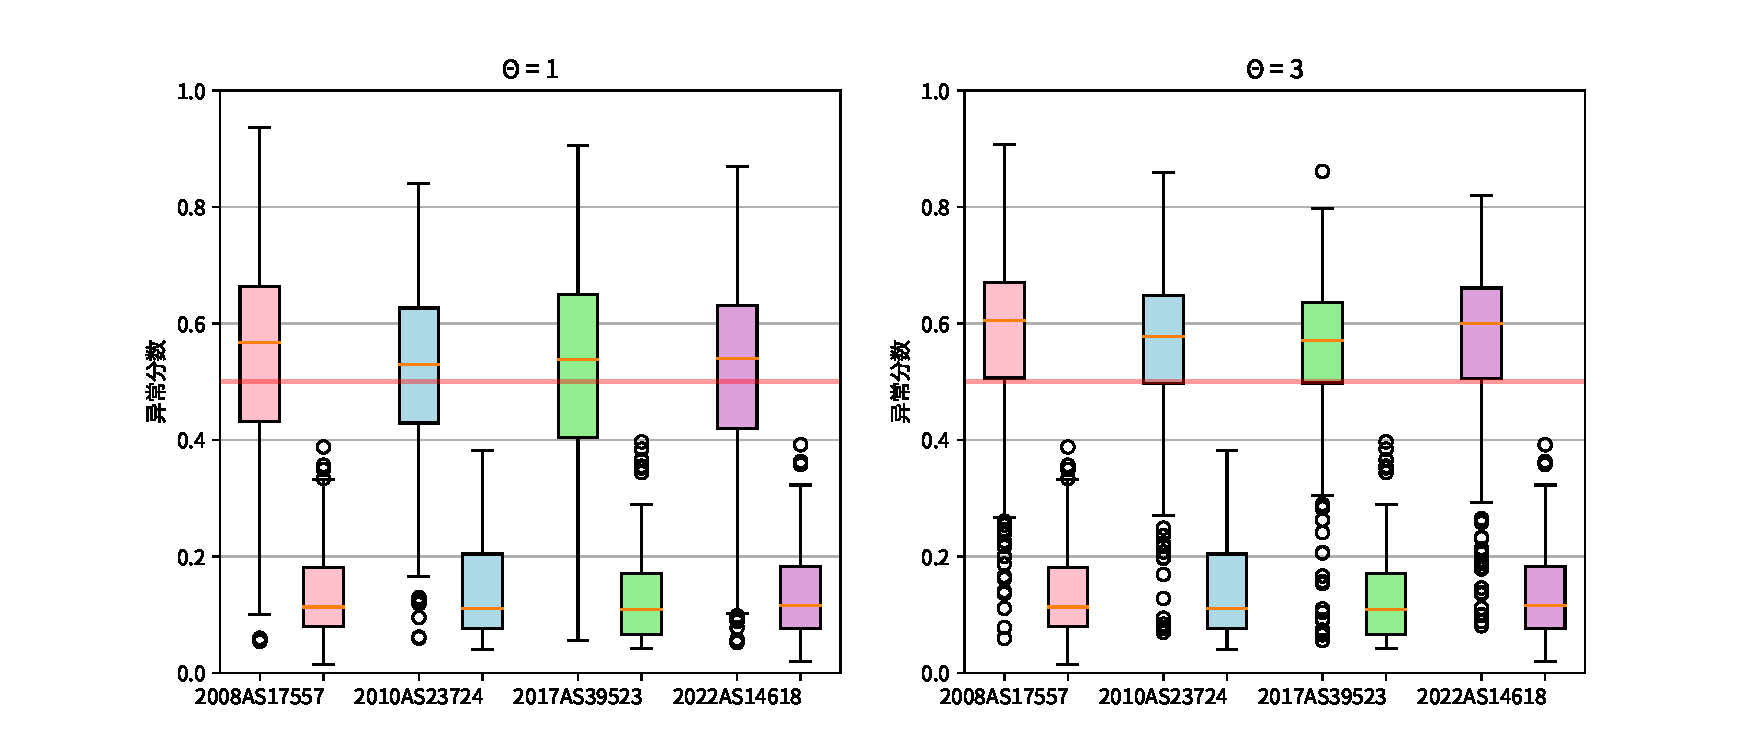
\includegraphics[width=\linewidth]{chapter/c5_images/c5_arg-analysis.pdf}
    \caption{参数分析结果}
    \label{c5_arg-analysis}
\end{figure}

% 对于 RIPE RIS 上的已知案例,通过调整参数确定参数与效果的关联。

\subsection{案例分析}

由于历史上具有标记、全球性的路由异常事件非常稀少,仅通过对已有路由异常的重放来测试模型的识别能力并不足够。因此,本文还设置了一组案例分析实验用于模拟真实的路由劫持事件,并由此分析模型在面对不同网络环境下路由异常的性能。

\subsubsection{实验设置}

本文在先前章节中提及了 DN42 的基本概况,它是一个社区构成的实验性网络,具有灵活的组网方式和具有相对较少限制的社区规范,这使得本实验能够实际生成具有劫持效果的 BGP 路由,并通过路由收集器(即 DN42 GRC)获取包含异常路由的数据集。

在此实验的预备工作中,本研究首先以自治系统 AS4242421332 的身份接入到 DN42 网络中,并将两个 IP 前缀通过 BGP 协议向 DN42 其它自治系统进行了宣告。在维持正常的网络路由一段时间后,正常的路由表能够被路由收集器收集并生成数据集文件,其中即包含了以该自治系统为起点到达网络中一部分自治系统的最优和次优路径集合。

随后,进行实验的异常路由部分,本实验在另一个能够控制的自治系统 AS4242421331 中以路径改写的方式,宣告一系列具有劫持效果的路由,意图将通往目标网络的流量劫持至该网络。此行为将被网络自身及其各阶邻居通告给路由收集器,随后以更新文件的形式将包含异常路由的路由表 MRT 文件生成出来。

异常检测模型将以这两个文件作为输入,输出对流量劫持开始后的 BGP 路由更新的异常检测分数。同样的,此实验按照 200\% 时间跨度,等比例地划分了 128 份路由更新数据。

\subsubsection{实验结果}

在获得了正确的异常检测输出后,本实验将路由嵌入的平均余弦距离与时间的关系以图表的方式输出,以便于分析模型检测路由异常后的输出是否稳定和合理。

\begin{figure}[h]
    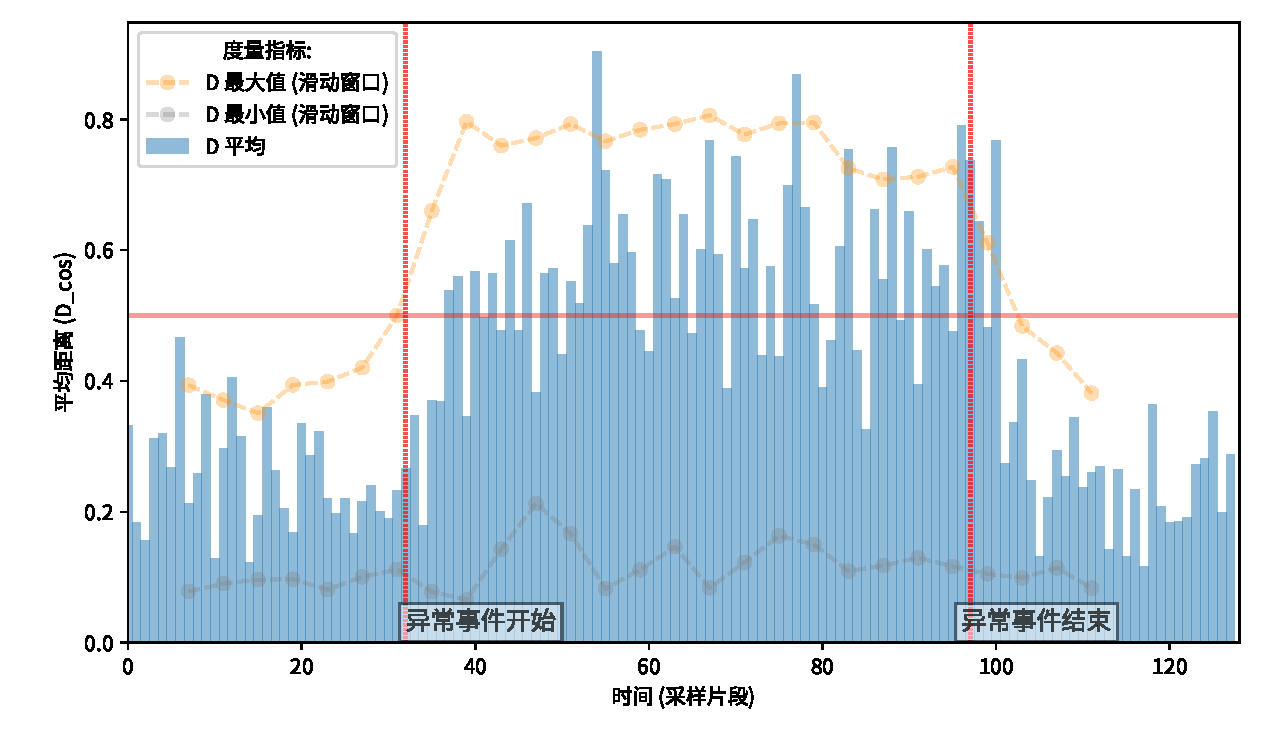
\includegraphics[width=\linewidth]{chapter/c5_images/c5_route-distance.pdf}
    \caption{时间序列上的特征距离分析}
    \label{c5_route-distance}
\end{figure}

如图 \ref{c5_route-distance} 显示,如使用 top-k 在一段时间分析路由异常的最大值或者平均值,模型是能够明确判断出路由异常的,以最大特征距离为标志的度量值在劫持发生后立即升高并突破 0.5 的阈值。此外,通过对比不同的指标可以观察到,特征距离最小值在整个事件中没有明显变化,一种可能的原因是 BGP 路由的更新在广域网络的邻居间相互传递,收敛较为缓慢,部分网络中存在的路由震荡抑制机制也使得突发的 BGP 更新无法及时反映到 GRC 的数据中,由于同样的原因,对于平均路由距离值而言,它相比异常的发生存在一定的延后时间。

通过 t-SNE 对异常发生前后的更新路径与原路径的表征进行降维,能够以此作出路径嵌入的可视化预览图,以分析此段时间内路由嵌入的状况,如图 \ref{c5_case-study-scatter},可见更新的路由被映射到了一个远离正常路径的区域(图中的红色区域)。值得注意的是,即使在未被标记为异常的时间段内的路由数据中,依然存在与异常数据较为接近或与其它路由更新距离较远的路由嵌入,这部分路由被认为是网络中偶发的拓扑改变所产生的背景噪声(图中的黄色区域是其中的一部分示例),这与参数分析中的图 \label{c5_arg-analysis} 的结果相对应。

\begin{figure}[h]
    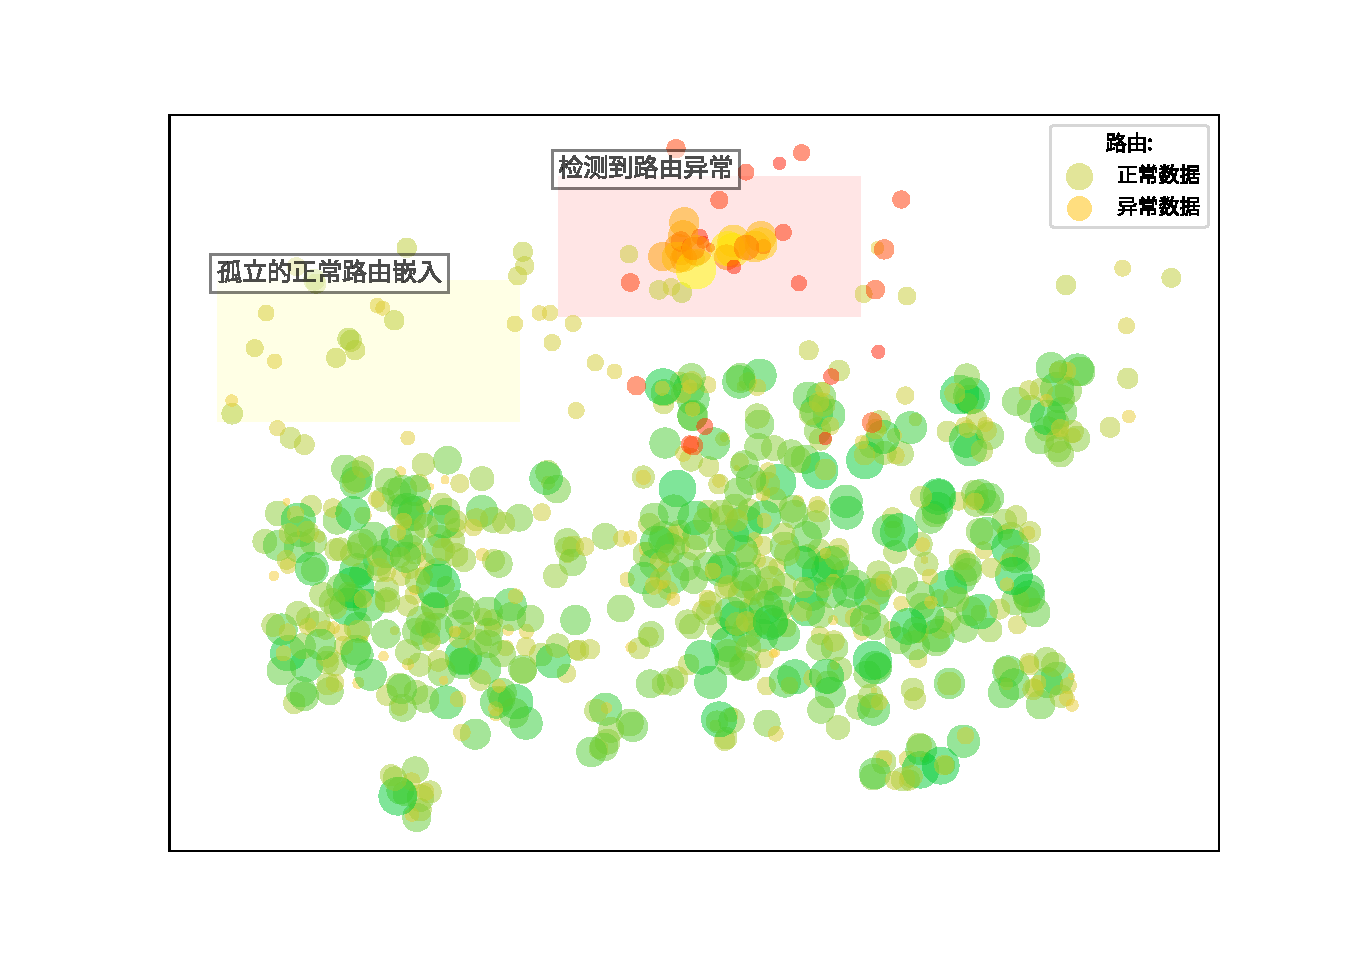
\includegraphics[width=\linewidth]{chapter/c5_images/c5_case-study-scatter.pdf}
    \caption{异常发生后的更新路径与原路径的表征}
    \label{c5_case-study-scatter}
\end{figure}
